% begin module higher-derivatives-ex6
\begin{frame}
\begin{example} %[Example 7, p. 153]
If $f(x) = x^3-x$, find $f''(x)$.
\begin{columns}[c]
\column{.4\textwidth}


\ 

\only<handout:0| 1>{%
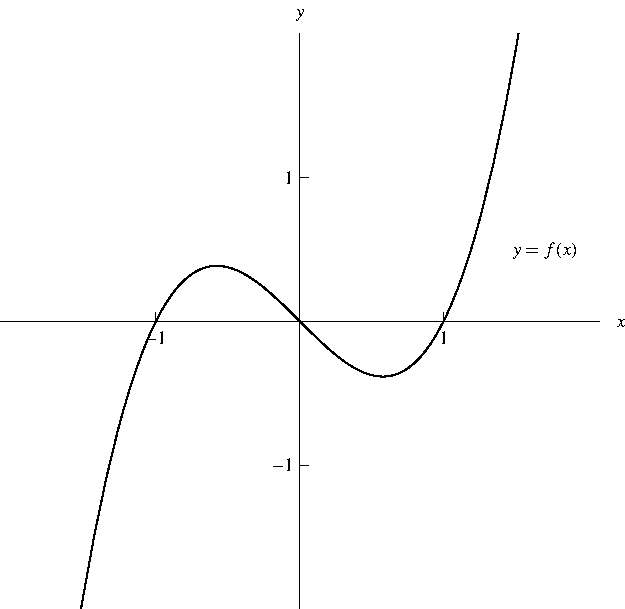
\includegraphics[height=4.5cm]{derivatives/pictures/03-02-ex6a.pdf}%
}%
\only<handout:0| 2-7>{%
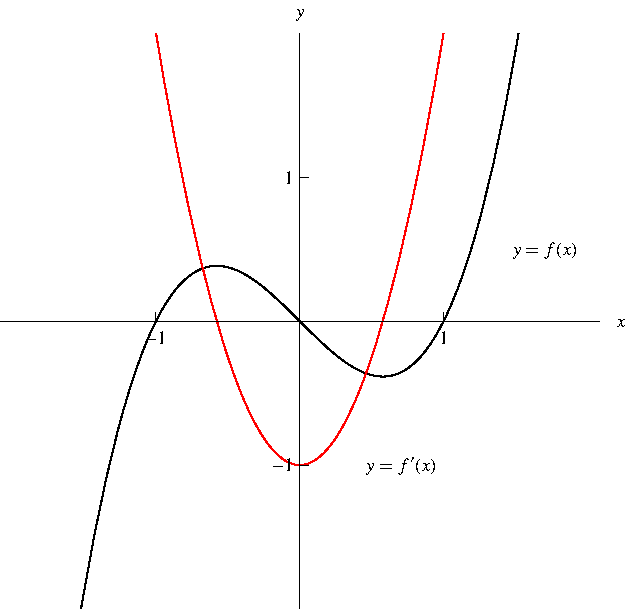
\includegraphics[height=4.5cm]{derivatives/pictures/03-02-ex6b.pdf}%
}%
\only<8->{%
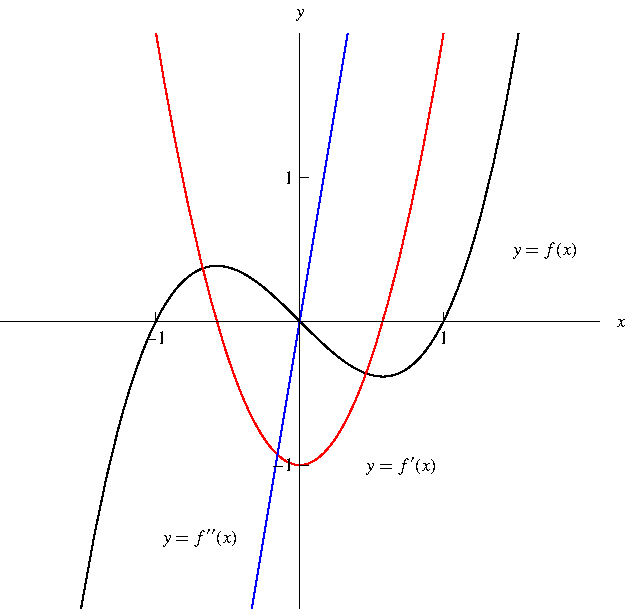
\includegraphics[height=4.5cm]{derivatives/pictures/03-02-ex6c.pdf}%
}%
\column{.6\textwidth}
\uncover<2->{%
In a previous exercise we found that the first derivative is $f'(x) = 3x^2 - 1$.
}%
\abovedisplayskip=0pt
\belowdisplayskip=0pt
\begin{align*}
&  \uncover<3->{f''(x)}\\%
 & \uncover<3->{ = }  %
\uncover<3->{\lim_{h\rightarrow 0}\frac{f'(x+h)-f'(x)}{h}}\\%
 & \uncover<4->{ = }  %
\uncover<4->{\lim_{h\rightarrow 0}\frac{[3(x+h)^2-1]-[3x^2-1]}{h}}\\%
 & \uncover<5->{ = }  %
\uncover<5->{\lim_{h\rightarrow 0}\frac{3x^2 + 6xh + 3h^2 -1 - 3x^2 +1}{h}}\\%
 & \uncover<6->{ = }  %
\uncover<6->{\lim_{h\rightarrow 0}\frac{6xh + 3h^2}{h}}\\%
 & \uncover<7->{ = }  %
\uncover<7->{\lim_{h\rightarrow 0}(6x + 3h)}\uncover<8->{ = 6x}%
\end{align*}
\end{columns}
\end{example}
\end{frame}
% end module higher-derivatives-ex6
